% To je predloga za poročila o domačih nalogah pri predmetih, katerih
% nosilec je Blaž Zupan. Seveda lahko tudi dodaš kakšen nov, zanimiv
% in uporaben element, ki ga v tej predlogi (še) ni. Več o LaTeX-u izveš na
% spletu, na primer na http://tobi.oetiker.ch/lshort/lshort.pdf.
%
% To predlogo lahko spremeniš v PDF dokument s pomočjo programa
% pdflatex, ki je del standardne instalacije LaTeX programov.

\documentclass[a4paper,11pt]{article}
\usepackage{a4wide}
\usepackage{fullpage}
\usepackage[utf8x]{inputenc}
\usepackage[slovene]{babel}
\selectlanguage{slovene}
\usepackage[toc,page]{appendix}
\usepackage[pdftex]{graphicx} % za slike
\usepackage{setspace}
\usepackage{color}
\definecolor{light-gray}{gray}{0.95}
\usepackage{listings} % za vključevanje kode
\usepackage{hyperref}

% Matlab code
\definecolor{mygreen}{RGB}{28,172,0} % color values Red, Green, Blue
\definecolor{mylilas}{RGB}{170,55,241}

\usepackage{amsmath}
\usepackage{siunitx}
\usepackage{eurosym}

\renewcommand{\baselinestretch}{1.2} % za boljšo berljivost večji razmak
\renewcommand{\appendixpagename}{Priloge}

\lstset{ % nastavitve za izpis kode, sem lahko tudi kaj dodaš/spremeniš
language=Python,
basicstyle=\footnotesize,
basicstyle=\ttfamily\footnotesize\setstretch{1},
backgroundcolor=\color{light-gray},
}

\lstset{language=Matlab,%
    %basicstyle=\color{red},
    breaklines=true,%
    morekeywords={matlab2tikz},
    keywordstyle=\color{blue},%
    morekeywords=[2]{1}, keywordstyle=[2]{\color{black}},
    identifierstyle=\color{black},%
    stringstyle=\color{mylilas},
    commentstyle=\color{mygreen},%
    showstringspaces=false,%without this there will be a symbol in the places where there is a space
    numbers=left,%
    numberstyle={\tiny \color{black}},% size of the numbers
    numbersep=9pt, % this defines how far the numbers are from the text
    emph=[1]{for,end,break},emphstyle=[1]\color{red}, %some words to emphasise
    %emph=[2]{word1,word2}, emphstyle=[2]{style},    
}


\title{Rešene izpitne naloge \\ 
	\large Optimizacijske Metode 2020/21}
\author{David Rubin}
\date{\today}

\begin{document}

\maketitle

\tableofcontents
\newpage


\section{Uvod}

Dokument predstavlja zapisnik dela, ki se je izvajalo na vajah predmeta. Poleg tega dokumenta so dostopne tudi podmape, v katerih se nahajajo \texttt{m file}, ki vsebujejo nekatere definicije za izvedbo ukazov, ki pripeljejo do ustreznih rešitev.

\section{Splošni napotki vaj}

\subsection{Termin 12.10.2020}

V kolikor uporabljaš simbolične funkcije, je potrebno spremenljivke inicializirati s \texttt{syms}. V kolikor bi si rad izrisal neko funkcijo, to storiš najlažje tako, da si definiraš simbolične spremenljivke s \texttt{syms}, definiraš neko funkcijo in kličeš izris s \texttt{ezmesh} (ali \texttt{fmesh}). Malo je treba tudi ugibati pri definiciji intervala, na katerem je izris, da dobiš dobro predstavitev. Glej kodo~\ref{vaje1splosno}

\lstinputlisting[label=vaje1splosno,caption=Splošna uporaba Matlab na 1. vajah,language=Matlab]{vaje1/vaje1.m}

Še nekaj koristnih napotkov pri uporabi funkcij:
\begin{itemize}
	\item \texttt{fminsearch(@($x$) function($x$), $x_0$)} ... Uporabimo, ko iščemo minimume funkcij. \texttt{@($x$)} nam pove, da je $x$ neodvisna spremenljivka. \texttt{function($x$)} je definicija neke funkcije (v večini primerov skozi ta dokument, bo ta funkcija shranjena v ločenem m-file). $x_0$ nam določa, kje bo postopek pričel, torej našo začetno točko. Priporočljivo je, da se uporabijo različne točke, saj se lahko nekatere \textit{ujamejo} v lokalne minimume, mi pa si želimo poiskati globalnega. Dovolj dobro je, da vzamemo kar nekaj naključno generiranih točk, si shranimo rešitve za vsak klic in jih med sabo primerjamo. Če so vse vrednosti enake, potem to tipično pomeni, da je algoritem našel globalni minimum v vseh primerih, rešitev je potem katerakoli izmed pridobljenih. V kolikor niso vse rešitve enake, pa vzamemo najmanjšo vrednost, saj je tam globalni minimum. Za iskanje maksimumov lahko uporabimo isto funkcijo in ji spremenimo le parametre: \texttt{fminsearch(@($x$) -function($x$), $x_0$)} (dodali smo -). Paziti je potrebno, da ima tudi rezultat potem spremenjen (negativen) predznak.
	
	\item \texttt{fmincon(@($x$) function($x$), $x_0$, $A$, $b$, $A_{eq}$, $b_{eq}$, LB, UB, NONLCON)} ... pa je funkcija, kjer išemo minimume ob podanih omejitvah. Enako kot prej sta defirnirani \texttt{function($x$)} in $x_0$, dodajo pa se še naslednji členi. Matrika $A$ predstavlja omejitve, pri katerih gre za relacijo $\leq$. V matriko $A$ zapišemo števila na levi strani pred spremenljivkami, paziti pa je potrebno, da če katera spremenljivka ni označena v omejitvi jo v matriki predstavimo s členom 0. Vektor $b$ predstavlja desno stran omejitev (torej vrednosti ki so na desni strani relacije $leq$). V kolikor je relacija $\geq$ je potrebno vse člene ustrezno pomnožiti z $-1$. Matrika $A_{eq}$ in vektor $b_{eq}$ predstavljata omejitve kjer je relacija $=$. \texttt{LB} in \texttt{UB} predstavljata spodnjo (\textit{Lower Bound}) in zgornjo mejo (\textit{Upper Bound}). \texttt{NONLCON} pa uporabimo kadar omejitve niso linearne (\textit{non linear constraints)}. V tem primeru se tipično definirajo v ločenem \textit{m-file}. Glej primer na nalogi TODO
\end{itemize}

Poglejmo si primer iskanja minimuma za funkcijo \texttt{bana} definirano v ločenem \textit{m-file}:
\lstinputlisting[label=minsearch_sample_function,language=Matlab]{vaje1/bana.m}
Uporabimo klic in določimo nek interval (pri tem lahko za enostavne funkcije pomaga izris):
\begin{lstlisting}[label=minsearch_sample_call,language=Matlab]
% Funkcija vraca tocko x, vrednost minimuma fval, in zastavico flag (katero opazujemo da je 1 - pomeni da je najdena ustrezna resitev)
[x, fval, flag] = fminsearch(@(x)bana(x), [-3, -3])
% Vrne:
%	x =[-2.7468   -2.7468]
%	fval = -100.1178
%	flag = 1
% Imamo se en lokalni minimum, ce ponovimo iskanje v drugi tocki
[x, fval, flag] = fminsearch(@(x)bana(x), [-3, 3])
% Vrne:
%	x =[-2.7468   2.9035]
%	fval = -128.3912
%	flag = 1
\end{lstlisting}


\section{Izpitne naloge}

V nadaljevanju sledijo izpitne naloge in postopki za pridobitev rešitev.
\newpage

\subsection{Izpit 23. maj 2008}

\subsubsection{Naloga 1.)}
\label{task:maj2008_1}

\textbf{Navodila:} \\ 
Minimiziraj funkcijo:

\begin{equation} \label{eq:maj2008_1}
f(x) = (x_1 - 0.5)^2 (x_1 + 1)^2 + (x_2 + 1)^2 (x_2 - 1)
\end{equation}
Ali ima funkcija samo en lokalni minimum oziroma maksimum? Če jih ima morda več, jih poišči! Kolikšna je vrednost funkcije v točki minimuma. Pomagaš si lahko z risanjem funkcije.
\textbf{Rešitev:} \\ 
Funkcijo si lahko izrišemo s pomočjo ukazov

\begin{lstlisting}[language=Matlab]
syms x y
f = (x - 0.5)^2 * (x + 1)^2 + (y + 1)^2 * (y - 1)^2;
fmesh(f, [-3, 3])
\end{lstlisting}
V novem \texttt{maj2008\_1.m} si definiramo funkcijo:
\lstinputlisting[language=Matlab]{vaje1/maj2008_1.m}
Potem lahko napišemo skripto (oziroma preverimo v zanki) iskanje minimuma iz večih točk:

\begin{lstlisting}[language=Matlab]
resitve = [];  % vnaprej pripravljen vektor resitev
for i=1:100  % 100 iteracij
	random_x0 = 20 * rand(1:2) - 10  % nakljucna zacetna tocka iz intervala [-10, 10]
	[x, fval, flag] = fminsearch(@(x)maj2008_1(x), random_x0)
	if flag == 1
		resitve = [resitve; [x fval]]  % shrani si dobre resitve
	end
end
b = uniquetol(resitve, 1e-6, 'byrows', true)  % izloci duplikatne resitve
% Vrne v stilu:
% b = 
%    -1.00  -1.00  0
%    -1.00   1.00  0
%     0.50   1.00  0
%     0.50  -1.00  0
\end{lstlisting}
Te unikatne rešitve so potem vrednosti za naše minimume. Prva dva stolpca sta vrednosti $x_1$ in $x_2$, tretji stolpec pa vrednost funkcije v tej točki $f(x_1, x_2)$.
Za iskanje maksimuma vidimo na grafu da je samo 1 in se nahaja v bližini točke $[0, 0]$, zato uporabimo le 1 klic:

\begin{lstlisting}
[x, fval, flag] = fminsearch(@(x)-maj2008_1(x), [0, 0])
% Vrne v stilu:
% x = [-0.2500    0.0000]
% fval = -1.3164
% flag = 1
\end{lstlisting}
Kar pomeni da je točka $[-0.25, 0]$ lokalni maksimum z vrednostjo -1.3164.


\subsubsection{Naloga 2.)}
\label{task:maj2008_2}

\textbf{Navodila:} \\
Maksimiziraj funkcijo in izračunaj njeno vrednost v točki maksimuma:
\begin{equation} \label{eq:maj2008_2}
f(x) = (x_1^2 + 2x_2^2)e^{-(x_1^2 + x_2^2)}
\end{equation}
\textbf{Rešitev:} \\
Podobno kot v nalogi~\ref{task:maj2008_1} si najprej narišemo funkcijo, in potem poskušamo identificirati število in postopek iskanja maksimumov:

\begin{lstlisting}[language=Matlab]
syms x y
f = (x^2 + 2*y^2) * exp( -(x^2 + y^2) );
fmesh(f, [-3, 3])
\end{lstlisting}

\begin{figure}[hbt]
\centering
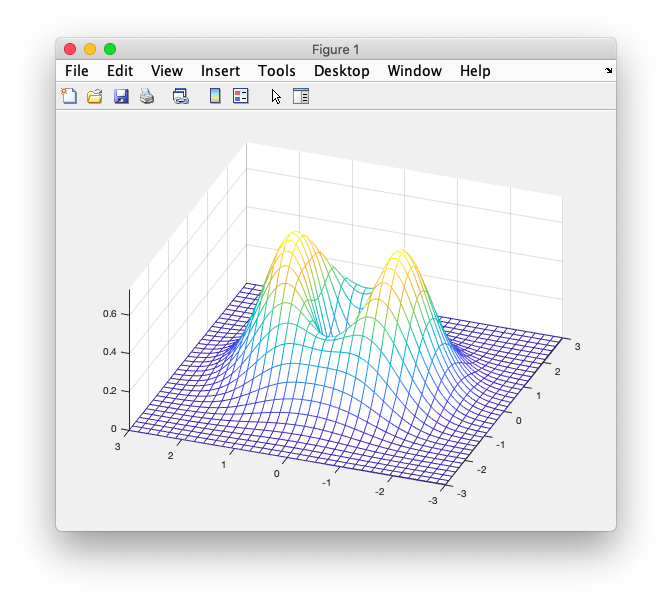
\includegraphics[scale=.4]{images/nal2_maj2008_plot.png}
\caption{Izris funkcije~\ref{eq:maj2008_2} na intervalu $[-3, 3]$.}
\label{img:maj2008_2_plot}
\end{figure}

Pri izrisu (glej sliko~\ref{img:maj2008_2_plot}) vidimo, da ima funkcija 2 vrhova in to v bližini točk $[0, -1]$ in $[0, 1]$. Funkcijo definiramo v ločenem \textit{m-file} (\texttt{maj2008\_2.m}):
\lstinputlisting[language=Matlab]{vaje1/maj2008_2.m} 
... in uporabimo informacijo iz izrisa v naslednjem klicu:
\begin{lstlisting}
[x, fval, flag] = fminsearch(@(x)-maj2008_2(x), [0, 1])
% Vrne v stilu:
% x =  [0    1]
% fval = -0.7358
% flag = 1
[x, fval, flag] = fminsearch(@(x)-maj2008_2(x), [0, -1])
% Vrne v stilu:
% x =  [0   -1]
% fval = -0.7358
% flag = 1
\end{lstlisting}
Točke, ki smo jih ocenili na grafu, so očitno maksimumi. Treba pa je paziti, saj je vrednost maksimumov v \texttt{fval} obratna - pravina vrednost obeh maksimumov je torej $f_{max} = 0.7358$.


\subsubsection{Naloga 3.)}
\label{task:maj2008_3}

\textbf{Navodila:} \\
Določi minimum funkcije in njeno vrednost v točki minimuma:
\begin{equation} \label{eq:maj2008_3}
f(x) = (x_1 - 2)^2 + (x_2 - 1)^2
\end{equation}
ob naslednjih omejitvah
\begin{equation} \label{con:maj2008_3}
\begin{aligned}
-x_1 -x_2 + 2 \geq 0 \\
-x_1^2 + x_2 \geq 0
\end{aligned}
\end{equation}
\textbf{Rešitev:} \\
Najprej si izrišimo funkcijo, da dobimo vpogled s čem imamo opravka (glej sliko~\ref{img:maj2008_3_plot}). Vidimo, da imamo 1 globalni minimum nekje relativno blizu točke $[0, 0]$.

\begin{figure}[hbt]
\centering
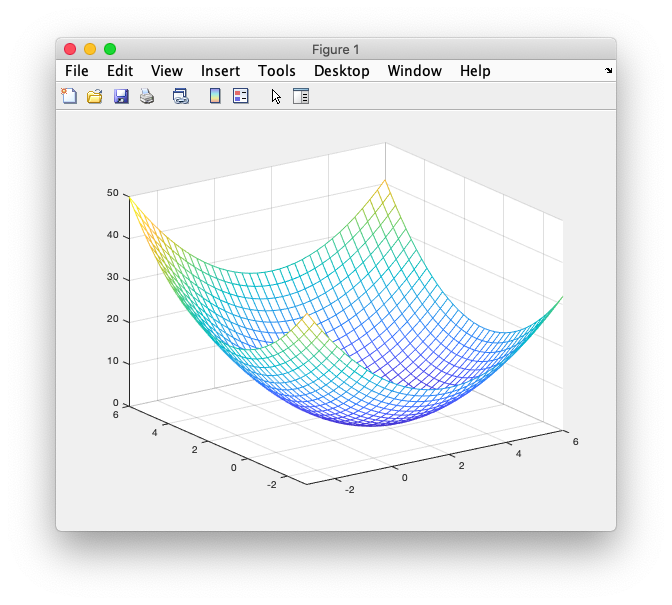
\includegraphics[scale=.4]{images/maj2008_3_plot.png}
\caption{Izris funkcije~\ref{eq:maj2008_3} na intervalu $[-3, 6]$.}
\label{img:maj2008_3_plot}
\end{figure}

V ločenem \textit{m-file} si sedaj definiramo funkcijo (\texttt{maj2008\_3.m}):
\lstinputlisting[language=Matlab]{vaje1/maj2008_3.m}
... in omejitve (\texttt{maj2008\_3\_con.m}):
\lstinputlisting[language=Matlab]{vaje1/maj2008_3_con.m}
Omejitve so tipa $\geq$, zato smo jih pomnožili s $-1$ preden smo jih vstavili v spremenljvko \texttt{c}. Sedaj lahko poženemo iskanje minimuma v bližini $[0, 0]$:
\begin{lstlisting}
[x, fval, flag] = fmincon(@(x)maj2008_3(x), [0, 0], [], [], [], [], [], [], @(x)maj2008_3_con(x))
% Vrne v stilu:
% x =  [1.000   -1.000]
% fval = 1.0000
% flag = 1
\end{lstlisting}
kar nam vrne rešitev $f_{min} = 1.000$ v točki $[1, -1]$.


\subsubsection{Naloga 4.)}
\label{task:maj2008_4}

\textbf{Navodila:} \\
Poišči vse ničle enačbe:
\begin{equation} \label{eq:maj2008_4}
f(x) = x^5 -6x^4 - 92x^3 + 402x^2 + 91x - 396
\end{equation}
\textbf{Rešitev:} \\
Uporabimo funkcijo \texttt{roots} in ji podamo koeficiente za vsako stopnjo $x$:
\begin{lstlisting}
roots([1 -6 -92 402 91 -396])
% Vrne v stilu:
% ans =
%    -9.0000
%    11.0000
%     4.0000
%    -1.0000
%     1.0000
\end{lstlisting}
Rešitev (ničle) so torej pri $x \in \{-9, -1, 1, 4, 11\}$


\subsubsection{Naloga 5.)}
\label{task:maj2008_5}

\textbf{Navodila:} \\
Letalska družba kupuje gorivo za letala pri treh različnih prodajalcih. Družba potrebuje v naslednjem mesecu na vsakem od treh letališč, kjer pristaja, naslednje količine goriva: $100.000 \si{\litre}$  na letališču 1, $180.000 \si{\litre}$ na letališču 2 ter $350.000 \si{\litre}$ na letališču 3. Gorivo prodajajo trije prodajalci, njihovo ceno goriva na posameznem letališču podaja naslednja tabela (cene so v centih na liter):
\begin{table}[hbt]
 	\centering
	\begin{tabular}{| l | c | c | c | }
		\hline
 			& Letališče 1 & Letališče 2  & Letališče 3 \\ \hline
		Prodajalec 1 & 92 & 89 & 90 \\ \hline
		Prodajalec 2 & 91 & 91 & 95 \\ \hline
		Prodajalec 3 & 87 & 90 & 92 \\ \hline
	\end{tabular}
\end{table}

Vsak prodajalec pa ima na voljo omejene količine goriva, ki ga skupno lahko dostavi v posameznem mesecu. Te količine so $320.000\si{\litre}$ prvi prodajalec, $270.000\si{\litre}$ drugi ter $190.000\si{\litre}$  tretji prodajalec. Določi pravilo za nakup goriva letalske družbe, ki bo zadovoljilo njihovim potrebam na vsakem od letališč ter bo ekonomsko čimbolj ugodno.

\textbf{Rešitev}: \\
Najprej si zastavimo spremenljivke $x_i,$ kjer  $i  \in \{1, 2, 3, 4, 5, 6, 7, 8, 9\}$, pri čemer je $x_1$ količina goriva kupljenega na letališču 1 pri prodajalcu 1, $x_2$ je količina goriva kupljenega na letališču 2 pri prodajalcu 1, ... in $x_9$ je količina goriva kupljenega na letališču 3 pri prodajalcu 3. Iz tega sledijo omejitve:

\begin{equation} \label{con:maj2008_5}
\begin{gathered}
x_1 + x_2 + x_3 \geq 320.000 \\
x_4 + x_5 + x_6 \geq 270.000 \\
x_7 + x_8 + x_9 \geq 190.000 \\
x_1 + x_4 + x_7 = 100.000 \\
x_2 + x_5 + x_8 = 180.000 \\
x_3 + x_6 + x_9 = 350.000 \\
x_1, x_2, x_3, x_4, x_5, x_6, x_7, x_8, x_9 \geq 0
\end{gathered}
\end{equation}
... in funkcija, ki jo minimiziramo:
\begin{equation} \label{eq:maj2008_5}
f(x) = 92x_1 + 89x_2 + 90x_3 + 91x_4 + 91x_5 + 95x_6 + 87x_7 + 90x_8 + 92x_9
\end{equation}
Vključili smo tudi omejitev nenegativnosti, saj smatramo, da letalska družba ne želi preprodajati goriva iz enega letališča na drugo (torej kupiti negativno količino). Problem lahko rešimo s funkcijo \texttt{intlinprog}:
\lstinputlisting[language=Matlab]{vaje1/maj2008_5.m}
Iz tega lahko razberemo, da je najugodneje na letališu 1 kupiti $100.000\si{\litre}$ pri prodajalcu 3, na letališču 2 $120.000\si{\litre}$ pri prodajalcu 2 in $60.000\si{\litre}$ pri prodajalcu 3, na letališču 3 pa $320.000\si{\litre}$ pri prodajalcu 1 in $30.000\si{\litre}$ pri prodajalcu 3. Skupno bomo porabili 565.800,00 \euro{}.


\subsection{Izpit 11. junij 2008}

\subsubsection{Naloga 1.)}
\label{task:junij2008_1}

\textbf{Navodila:} \\
Poišči vse lokalne ekstreme funkcije na intervalu $[-3, 3]$ in njene vrednosti v teh točkah:
\begin{equation} \label{eq:junij2008_1}
f(x) = \frac{1}{2}( \sin(5x) - x)^2
\end{equation}
\textbf{Rešitev:} \\
Izrišimo funkcijo:

\begin{figure}[hbt]
\centering
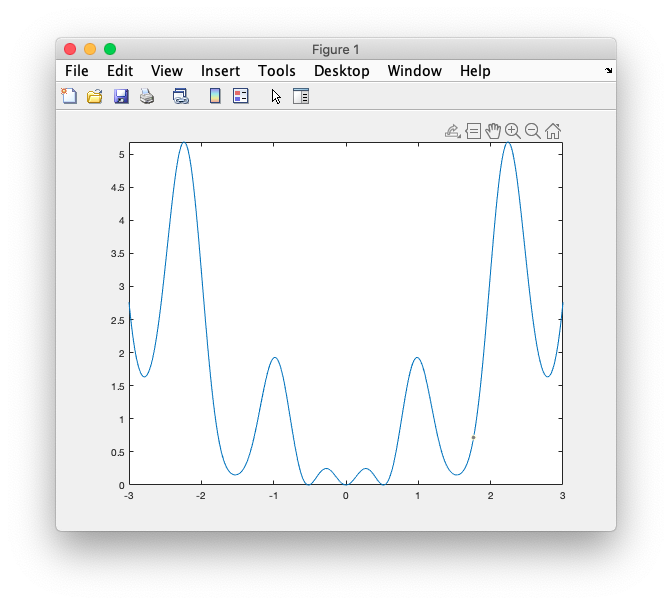
\includegraphics[scale=.4]{images/junij2008_1_plot.png}
\caption{Izris funkcije~\ref{eq:junij2008_1} na intervalu $[-3, 3]$.}
\label{img:junij2008_1_plot}
\end{figure}
Vidimo, da imamo 7 lokalnih minimumov in 6 lokalnih maksimumov. \textbf{TODO}


\subsubsection{Naloga 2.)}
\label{task:junij2008_2}

\textbf{Navodila:} \\
Reši naslednji sistem enačb:
\begin{equation} \label{eq:junij2008_2}
	\begin{gathered}
		\sin(x + y) = 0 \\
		\cos(x - y) = 0
	\end{gathered}
\end{equation}
\textbf{Rešitev:} \\
V novem \textit{m-file} si definiramo enačbi (\texttt{junij2008\_2.m}):
\lstinputlisting[language=Matlab]{vaje2/junij2008_2.m}
... in nato kličemo funkcijo \texttt{fsolve}:
\begin{lstlisting}[language=Matlab]
% Poskusimo najprej s [0, 0]
x = fsolve(@(x)junij2008_2(x), [0, 0])
% Kar vrne, da ni resitve ...
% Premaknimo se v negativni del
xL = fsolve(@(x)junij2008_2(x), [-.5, -.5])
% ... in v pozitivni
xR = fsolve(@(x)junij2008_2(x), [.5, .5])
% In dobimo najmanjsi resitvi (ostale so periodicne)
% xL = 	[0.7854    -0.7854]
% xR =  [-0.7854    0.7854]
\end{lstlisting}
Rešitev so torej točke $x_1 = \frac{\pi}{4}$, $y_1 = -\frac{\pi}{4}$ in $x_2 = -\frac{\pi}{4}$, $y_2 = \frac{\pi}{4}$. Rešitve se periodično ponavljajo vsake $\frac{\pi}{2}$.

\subsubsection{Naloga 3.)}
\label{task:junij2008_3}

\textbf{Navodila:} \\
Določi minimum funkcije in njeno vrednost v točki minimuma:
\begin{equation} \label{eq:junij2008_3}
f(x) = x_1^2 + 5x_2^2 + 10x_3^2 - 4x_1x_2 + 6x_1x_3 - 12x_2x_3 - 2x_1 + 10x_2 - 5x_3
\end{equation}
ob naslednjih omejitvah:
\begin{equation} \label{con:junij2008_3}
	\begin{gathered}
		x_1 + 2x_2 + x_3 \geq 4 \\
		x_1, x_2, x_3 \geq 0
	\end{gathered}
\end{equation}
\textbf{Rešitev:} \\
V novem \textit{m-file} si definiramo funkcijo (\texttt{junij2008\_3.m}):
\lstinputlisting[language=Matlab]{vaje2/junij2008_3.m}
In kličemo funkcijo \texttt{fmincon}:
\begin{lstlisting}[language=Matlab]
[x, fval] = fmincon(@(x)junij2008_3(x), [1 1 1], [-1 -2 -1], -4, [], [], [0 0 0])
% Vrne v stilu:
% x = [2.9412    0.5294    0.0000]
% fval = 3.2353
\end{lstlisting}
Začnemo v naključni točki $[1, 1, 1]$, omejitve (matrika $A$ in vektor $b$) morajo upoštevati relacijo $\leq$, zato so vrednosti obratne, $A_{eq}$ in $b_{eq}$ pustimo prazne, nastavimo pa še spodnjo mejo z $[0, 0, 0]$.
Rešitev je torej točka $x_{min} = [2.9412, 0.5294, 0.0000]$, v kateri imamo vrednost $f(x_{min}) = 3.2353$


\subsubsection{Naloga 4.)}
\label{task:junij2008_4}

\textbf{Navodila:} \\
Poišči minimum funkcije in njeno funkcijsko vrednost v točki minimuma:
\begin{equation} \label{eq:junij2008_4}
	f(x) = 2x_1^2 - x_1x_2 + x_2^2 - 3x_1 + e^{2x_1 + x_2}
\end{equation}
\textbf{Rešitev:} \\
Ker imamo le 2 spremenljivki, si izrišimo funkcijo (glej sliko~\ref{img:junij2008_4_plot}). 

\begin{figure}[hbt]
	\centering
	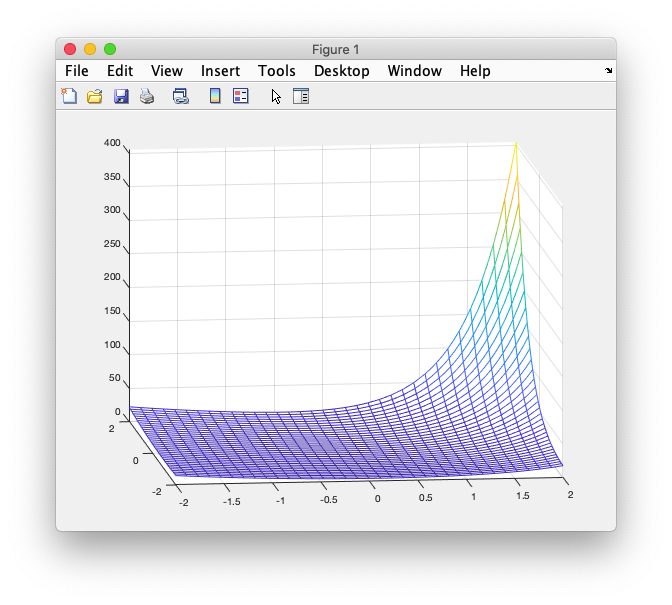
\includegraphics[scale=.4]{images/junij2008_4_plot.png}
	\caption{Izris funkcije~\ref{eq:junij2008_4} na intervalu $[-2, 2]$.}
	\label{img:junij2008_4_plot}
\end{figure}
Vidimo, da je nekje v bližini točke $[0, 0]$ morda minimum. Deifinirajmo nov \textit{m-file} (\texttt{junij2008\_4.m}):
\lstinputlisting[language=Matlab]{vaje2/junij2008_4.m}
... in kličemo funkcijo \texttt{fminsearch}:

\begin{lstlisting}[language=Matlab]
[x, fval, flag] = fminsearch(@(x)junij2008_4(x), [0, 0])
% Vrne v stilu:
% x = [0.1737   -0.3915]
% fval = 0.7174
% flag = 1
\end{lstlisting}
... ki nam poda našo rešitev: $x_{min} =  [0.1737, -0.3915]$, $f(x_{min}) = 0.7174$.

\subsubsection{Naloga 5.)}
\label{task:junij2008_5}

\textbf{Navodilo:} \\
Trgovina z malimi živalmi je ugotovila, da potrebuje hrček najmanj 70 enot beljakovin, 100 enot ogljikovih hidratov ter 20 enot maščob dnevno. Trgovina ima na zalogi 6 različnih vrst hrane za hrčke z naslednjimi lastnostmi:
\begin{table}[h]
	\centering
	\begin{tabular}{| c | c | c | c | c |}
		\hline
		Hrana & Beljakovin/dozo & Ogljikovih hidratov/dozo & Maščob / dozo & Cena / dozo \\ \hline
		A & 20 & 50 & 4 & 2 \\ \hline
		B & 30 & 30 & 9 & 3 \\ \hline
		C & 40 & 20 & 11 & 5 \\ \hline
		D & 40 & 25 & 10 & 6 \\ \hline
		E & 45  & 50 & 9 & 8 \\ \hline
		F & 30 & 20 & 10 & 8 \\ \hline
	\end{tabular}
\end{table}
Kakšno razmerje posameznih vrst hrane bo mešanica hrane za hrčka, ki bo zadovoljila njegove dnevne potrebe in bo cenovno najbolj ugodna za trgovino? Napiši sistem enačb in ga reši z MATLAB-om!

\textbf{Rešitev:} \\
Najprej določimo spremenljivke: $x_N$, kar pomeni koliko doz hrane $N$ bomo kupili ($N$ predstavlja vrsto hrane, torej A, B, C ... F). Funkcija ki jo minimiziramo je cena:
\begin{equation} \label{eq:junij2008_5}
f(x) = 2x_1 + 3x_2 + 5x_3 + 6x_4 + 8x_5 + 8x_6
\end{equation}
omejitve pa so sledeče:
\begin{equation}
	\begin{gathered}
		20x_1 + 30x_2 + 40x_3 + 40x_4 + 45x_5 + 30x_6 \geq 70 \\
		50x_1 + 30x_2 + 20x_3 + 25x_4 + 50x_5 + 20x_6 \geq 100 \\
		4x_1 + 9x_2 + 11x_3 + 10x_4 + 9x_5 +  10x_6 \geq 20 \\
		x_1, x_2, x_3, x_4, x_5, x_6  \geq 0
	\end{gathered}
\end{equation}
Enačno lahko rešimo s pomočjo funkcije  \texttt{intlinprog}:
\lstinputlisting[language=Matlab]{vaje2/junij2008_5.m}
Ugotovimo, da je cenovno najbolj ugodno kupiti 0.9091 doz hrane A in 1.8182 doz hrane B za skupno ceno 7.2727.


\subsection{Izpit 3. september 2008}
\subsubsection{Naloga 1.)}

\textbf{Navodila:} \\ 
Poišči vse lokalne minimume in maksimume funkcije na intervalu ter njene vrednosti v teh točkah. Pomagaš si lahko z risanjem funkcije. Ali obstaja globalni maksimum?
\begin{equation} \label{eq:september2008_1}
	f(x) = 3x_1x_2 + 40x_1 + 30x_2 - 4x_1^2  - x_1^4 -3x_2^2 -x_2^4
\end{equation}

\textbf{Rešitev:} \\
Najprej si narišimo funkcijo (slika~\ref{img:september2008_1_plot}).

\begin{figure}[hbt]
	\centering
	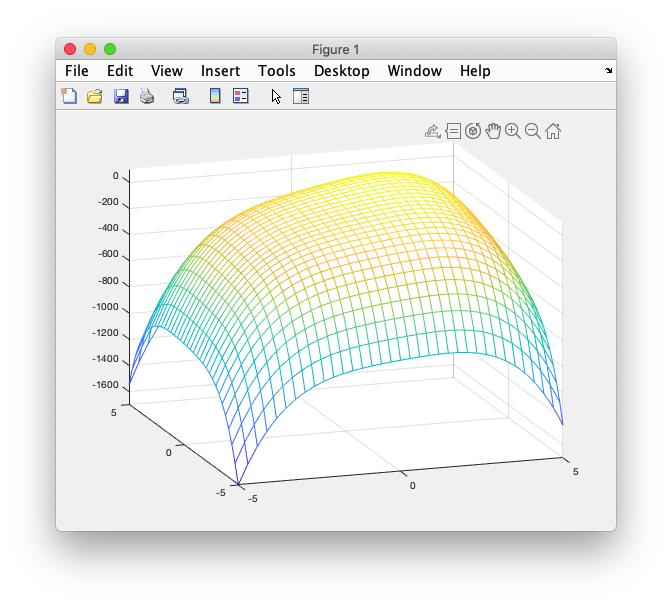
\includegraphics[scale=.4]{images/september2008_1_plot.png}
	\caption{Izris funkcije~\ref{eq:september2008_1} na intervalu $[-5, 5]$.}
	\label{img:september2008_1_plot}
\end{figure}
Iz grafa je razvidno, da imamo opravka z 1 globalnim maksimumom, ki ga poiščemo s \texttt{fminsearch}. Deifiniramo si funkcijo v ločenem \textit{m-file} (\texttt{september2008\_1.m}):
\lstinputlisting[language=Matlab]{vaje2/september2008_1.m}
... in pokličemo funkcijo v okolici $[-3, -3]$:
\begin{lstlisting}[language=Matlab]
[x, fval] = fminsearch(@(x)-september2008_1(x), [-3, -3])
% Vrne v stilu:
% x = [1.9548    1.8380]
% fval = -92.6766
\end{lstlisting}
Ne smemo pozabiti, ker smo obrnili predznak za maksimizacijo, je obrnjen tudi predznak vrednosti. Pravilna rešitev je torej pri $x_{max} = [1.9548, 1.8380]$ z vrednostjo $f(x_{max}) = 92.6766$.


\subsubsection{Naloga 2.)}

\textbf{Navodila:} \\ Maksimiziraj funkcijo in izračunaj njeno vrednost v točki maksimuma:
\begin{equation} \label{eq:september2008_2}
	f(x) = -(x_1 - x_2)^2 - (x_3 - 1)^2 - 1 - 0.02(x_1^5 + x_2^5 + x_3^5 - 16)^2
\end{equation}

\textbf{Rešitev:} \\
Funkcija ima preveč dimenzij za risanje, zato kar poskusimo z nekaj sreče. Definiramo si nov \textit{m-file} (\texttt{september2008\_2.m}:
\lstinputlisting[language=Matlab]{vaje2/september2008_2.m}
... in kličemo funkcijo \texttt{fminsearch} (z obratno vrednostjo ker maksimiziramo):
\lstinputlisting[language=Matlab]{vaje2/september2008_2_script.m}
Ker smo v tem primeru iskali maksimum funkcije, lahko rezultat sortiramo kar naraščujoče, saj je potrebno spremeniti predznak in je najmanjša vrednost enaka največi.
Vidimo, da je prvih 10 najdenih točk identičnih, torej lahko vzamemo maksimum $x_{max} = [1.4963, 1.4963, 1.0000]$ in vrednost $f_{max} = -1$ (ne pozabimo na $-$).


\subsubsection{Naloga 3.)}

\textbf{Navodila:} \\
Določi minimum funkcije in njeno vrednost v točki minimuma:
\begin{equation} \label{eq:september2008_3}
 	f(x) = 2x_1 +x_2^3 + x_3^2
\end{equation}
ob naslednjih omejitvah:
\begin{equation} \label{con:september2008_3}
	\begin{gathered}
		x_1^2 + 2x_2^2 +x_3^2 \geq 4
		x_1, x_2, x_3 \geq 0
	\end{gathered}
\end{equation}

\textbf{Rešitev:} \\
V ločenih \textit{m-file} si definiramo funkcijo (\texttt{september2008\_3.m}):
\lstinputlisting[language=Matlab]{vaje2/september2008_3.m}
... in omejitve (\texttt{september2008\_3\_con.m}):
\lstinputlisting[language=Matlab]{vaje2/september2008_3_con.m}
... in kličemo funkcijo \texttt{fmincon}:
\begin{lstlisting}
[x, fval, flag] = fmincon(@(x)september2008_3(x), [1 1 1], [], [], [], [], zeros(1, 3), [], @(x)september2008_3_con(x))
% Vrne v stilu:
%  x = [0.0000    1.3333    0.6667]
%  fval = 2.8148
%  flag = 1
\end{lstlisting}
Matrike $A, b, A_{eq}, B_{eq}$ smo pustili prazne, dodali smo spodnjo mejo ničel, zgornjo mejo nedefinirano in podali omejitve v ločenem \textit{m-file}.
Pridobljena rešitev je očitno veljavna (\texttt{flag = 1}): $x_{min} = [0.0000, 1.3333, 0.6667]$, vrednost pa je $f(x_{min}) = 2.8148$.


\subsection{Izpit 10. februrar 2014}

\subsubsection{Naloga 1.)}

Glej sliko na desktop.
Funkcija je definirana v testf4.m, skripta za zaganjane pa v script1.m

klicemo script1 in dobimo 999 resitev.
ressort = sortrows(resitve, 3) .. sortiramo

nekaj je mutil z unique, pa je dobil za vse vrstice 

- 186.7309 3 stolpec

enovite = unique(ressort(1:20,:))

\subsubsection{Naloga 2.)}

2 m file, pa se eno skripto si lahko naredis slika na namizju

\subsubsection{Naloga 3.)}

Geometrijska naloga, prisekan stožec ima špic odrezan. Skica: krog v njega narises trapez, po tem si nastavis enacbe za omejitev (stranski ris) slika na namizju


\subsubsection{Naloga 4.)}

gle jslika na namizju. Izdelki so nedeljivi -> pomeni da nastavis integer solutions. Modificiran knapsack problem (izdelki se lahko ponavljajo). Napisati si je treba enacbe (4 spremenljivke, koliko izdelkov P1 = x1, ...).
Cena 13x1  +27x2 ... + 55x4 - maksimiziras
Omejitve .... 21 ton + celan stevila (intlinprog, inlincon -> [1 2 3 4] ... vse morajo bit celostevilcne) 


\end{document}
